\documentclass{bioinfo}
\usepackage{url}
\usepackage{graphicx}
\usepackage{float}
\usepackage[colorlinks=true, citecolor=blue, linkcolor=blue, urlcolor=blue]{hyperref}
\usepackage{listings}

\copyrightyear{2015}
\pubyear{2015}

\definecolor{codegreen}{rgb}{0,0.6,0}
\definecolor{codegray}{rgb}{0.5,0.5,0.5}
\definecolor{codepurple}{rgb}{0.58,0,0.82}
\definecolor{backcolour}{rgb}{0.95,0.95,0.92}
 
\lstdefinestyle{mystyle}{
    backgroundcolor=\color{backcolour},   
    commentstyle=\color{codegreen},
    keywordstyle=\color{magenta},
    numberstyle=\tiny\color{codegray},
    stringstyle=\color{codepurple},
    basicstyle=\footnotesize,
    breakatwhitespace=false,         
    breaklines=true,                 
    captionpos=b,                    
    keepspaces=true,                 
    numbers=left,                    
    numbersep=5pt,                  
    showspaces=false,                
    showstringspaces=false,
    showtabs=false,                  
    tabsize=2
}
\renewcommand{\lstlistingname}{Code example}
 
\lstset{style=mystyle}

\begin{document}
\firstpage{1}

\title[short Title]{Bahavioral Design Patterns}
\author[Malte Brockmann, Jun-Heui Cho]{Malte Brockmann, Jun-Heui Cho}
\address{Department of Bioinformatics, Technische Universit\"at M\"unchen}

\history{}

\editor{}

\maketitle

\begin{abstract}
This report introduces the behavioral design patterns in general and describes two of many frequently used behavioral patterns, Memento pattern and Observer pattern, in detail. In particular, it will describe the pattern's functionality, its uses and drawbacks. To underline the presented patterns, the report will also show some implementations with the aid of example JavaScript projects by refactoring these projects with the patterns.
\end{abstract}

\section{Introduction}
Behavioral patterns are a subcategory of Design Pattern which are popular in software development. They are mainly implemented in object oriented programming languages. This might speak against the use of those pattern in JavaScript, caused by it's structure for example the use of prototyping as it's  inheritance structures. This report will show that it is possible to implement design or in particular behavioral patterns in JavaScript with some adjustments. Some behavioral patterns will be explained and applied to existing projects from "GitHub.com" \cite{github}.

The research  based on three main sources: The web page "dofactory.com" \cite{dofac} which provided explanations and JavaScript examples for all patterns. The web page "sourcemaking.com" \cite{sourcem} which contained further information  and abstract examples, but no implementation examples in JavaScript. The third main source is the book "Elements of Reusable Object-Oriented Software" by the authors which are called the "Gang of Four". \cite{gang4} This book provides basic information about design patterns. 

\section{Behavioral Design Patterns}

Behavioral patterns is one of the three groups of design patterns (creational, structural and behavioral). The behavioral patterns are: Chain of Responsibility, Command, Interpreter, Iterator, Mediator, Memento, Observer, State, Strategy, Template Method and Visitor pattern. Those can be divided into two subcategories, the behavioral class patterns and the behavioral object patterns. Class patterns use inheritance to distribute behavioral between classes, for example the Template Method. The object patterns in comparison use object compositions rather than inheritance.  They are concerned with how object corporations can handle tasks which a single object could not handle by itself (e.g. Mediator pattern). Furthermore these patterns try to encapsulate behavior from an object and delegate requests to it (e.g. Command pattern). \cite{gang4}
In summary behavioral patterns are concerned with algorithms and the assignment of responsibilities between objects. The patterns describe the communication between objects or classes and try to simplify complex control flows.
Inheritance play a significant role in the context of behavioral pattern which as mentioned earlier might be a problem regarding JavaScript, because it do not support inheritance in the way conventional object oriented languages do. JavaScript only supports prototype inheritance which is mainly used for sharing the same methods cause by the fact that there is no overriding of methods.
Despite this it is still possible to use behavioral patterns in JavaScript if the patterns are adjusted in certain ways.

\section{Memento Pattern}
"Without violating encapsulation, capture and externalize an object's internal state so that the object can be returned to this state later." \cite{sourcem} Simply put saving an object's (or a portion of it's) state, which can be restored later. This pattern is also used to provide a undo or a rollback functionality to a application. When applying the Memento pattern, it  is important to secure the rules of encapsulation, otherwise it is possible that the application's reliability and extensibility is compromised. \cite{gang4} 
%figures
\begin{figure}[ht]
    \centering
    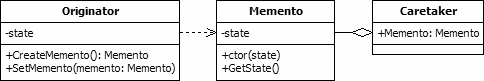
\includegraphics[width=1\linewidth]{img/Memento.png}
    \caption{UML diagram of the Memento pattern \cite{mementoUML}}
    \label{fig:Memento_pattern}
\end{figure}
\subsection{Participants}
To implement this pattern three participants are necessary. First we need the Originator which is the class whose state should be stored. It should include methods to create a memento of the Originator's current state. Furthermore it should have the ability to set the state to a memento which was stored earlier.
Second we need the Memento class itself which contains the information of the state of the Originator. The Memento has no influence on content or the amount which is being stored, this is completely controlled by the Originator. But the Memento can protect the stored states by providing no interface to modify the data. The only mandatory functionality is the ability to return the saved state.
The last participant is the caretaker whose sole function is to store Mementos.The caretaker can hold one or many Mementos, depending on the implementation, so multi-level undo and redo actions are possible. \cite{gang4}
\subsection{Collaboration}
As the diagram in figure~\ref{fig:Memento_pattern_sequence} shows, the Caretaker request a Memento from the Originator and holds it until passing it back to the Originator.
%figures
\begin{figure}[ht]
    \centering
    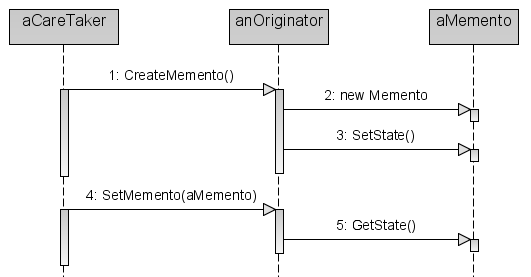
\includegraphics[width=1\linewidth]{img/Memento_design_pattern_sequence1.png}
    \caption{UML sequence diagram of the Memento pattern \cite{memento_seq}}
    \label{fig:Memento_pattern_sequence}
\end{figure}
\subsection{Use}
The Memento pattern is used to protect the information which only the Originator should have access to but should still be stored outside of the Originator. Furthermore the Originator itself is simplified when the work of storage management is not its responsibility. \cite{gang4}  

\subsection{Drawback}
If the information which should be stored to the Memento is large and the probability of a rollback is low, the Memento pattern gets expensive which can make the pattern inefficient. It is advisable to use this pattern only if encapsulating and restoring of the Originator's state is relatively cheap. For a basic implementation of this pattern, the storage cost of different Mementos in the Caretaker can get problematic if the Caretaker do not know when or how to delete unused Mementos. \cite{gang4}

\section{Observer Pattern}
The Observer pattern is a behavioral pattern used to define a one-to-many relationship between objects, so that as soon as one object changes its state, all its dependents are notified and updated automatically \cite{sourcem}. This means that no further action is needed for the one object who is sending out the notifications, and the dependent objects are to handle their own updates accordingly.

\subsection{Participants}

\begin{figure}[ht]
    \centering
    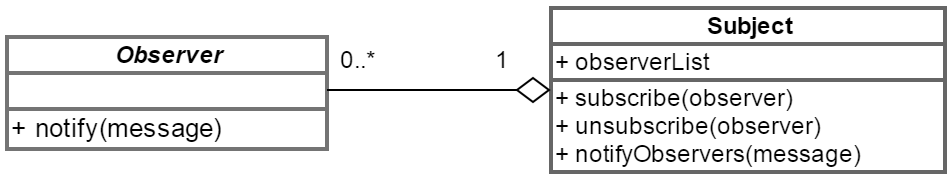
\includegraphics[width=1\linewidth]{img/observer-uml.png}
    \caption{Simplified UML diagram of the Observer pattern}
    \label{fig:Observer_pattern}
\end{figure}

For the Observer pattern, only two types of participants are necessary, namely the Subject and the Observer.

The Subject, on the one hand, is the one object that will notify the Observers about its state changes. It should have a subscription functionality for an Observer to be able to subscribe (and unsubscribe) to the Subject and thereby \textit{'observe'} the Subject. This way the Subject maintains a list of Observers that has subscribed to it. Furthermore, it needs a method to notify its Observers. This method loops through its Observers and call one of the Observers’ according notify methods. The notification usually contains a message as a parameter, so that the Observer knows how to react accordingly. \cite{dofac}

The Observer, on the other hand, only needs the mentioned notify method that can be invoked from the Subject with a message.

%Pic bla

\subsection{Use}
The Observer pattern is widely used in computer games. Most of the time, there are multiple objects and participants in games, where a single change in state – e.g. a players input or an event – will cause many other object to update their state as well.

The Observer pattern also finds a frequent use in GUIs (graphical user interfaces). For example, if a button is clicked by a user resulting in a state change, various GUI elements and views might need to adapt accordingly. \cite{wiki:observer}

\subsection{Drawback}
Sending notifications with messages to all observers can lead to high performance costs. Especially, if not every Observer has to react to every notification, it adds redundant costs.

With the standard implementation, it is not possible for the Subject to control the order of Observer notifications. This can cause problems in application where the update order of various objects is crucial. One could implement such a behavior by extending the Observer pattern, but this could lead to even more cost inefficiency.


\section{Refactored Projects}
In the following the earlier explained patterns will be implemented in form of a refactoring. The projects are accessible through a Github repository \cite{github}.

The first project is a implementation of a Space Invader game which will show the use of the Memento pattern.

The second project will refactor the game Pac-Man with the use of the Observer pattern.


\subsection{SpaceInvaders}
The Space Invader game is a single player JavaScript web based browser game. \cite{spaceinv} The game is a two-dimensional fixed shooter game in which the player tries to defeat five rows of ten aliens. The player is a cannon which can move horizontally across the bottom of the screen and shoot the invaders. The aliens try to destroy the cannon by firing at the cannon and moving towards the bottom of the screen. If they reach the bottom or if they hit the cannon three times the game ends. If the cannon destroys all the aliens a new wave of aliens appears which moves faster, which can be an endless loop. \cite{wiki:spaceinvader}       
This particular implementation works with different stages: The \texttt{WelcomeState}, \texttt{GameOverState}, \texttt{PlayState}, \texttt{PauseState} and the \texttt{LevelIntroState}. The states will be switched with the \texttt{moveState()} method.
The issue which will be addressed with the Memento pattern is the creation of new state objects instead of using already existing objects. As you can see in code example~\ref{code:spaceinvader_before_G} the \texttt{GameOverState} moves the state to a new \texttt{LevelIntroState} instead of using the state which was created in the \texttt{WelcomeState} (Code example~\ref{code:spaceinvader_before_W}). The difference that the \texttt{LevelIntroState} is created with the parameter \texttt{game.level} instead of 1 is irrelevant because \texttt{game.level} is always set to 1 in \texttt{WelcomeState}.

\begin{lstlisting} [caption=\texttt{WelcomeState} before the Memento pattern was applied, label=code:spaceinvader_before_W]
WelcomeState.prototype.keyDown = function(game, keyCode) {
    if(keyCode == 32) /*space*/ {
        //  Space starts the game.
        game.level = 1;
        game.score = 0;
        game.lives = 3;
        game.moveToState(new LevelIntroState(game.level));
    }
};
\end{lstlisting}

\begin{lstlisting} [caption=\texttt{GameOverState} before the Memento pattern was applied, label=code:spaceinvader_before_G]
GameOverState.prototype.keyDown = function(game, keyCode) {
    if(keyCode == 32) /*space*/ {
        game.lives = 3;
        game.score = 0;
        game.level = 1;
        game.moveToState(new LevelIntroState(1));
    }
};
\end{lstlisting}

To avoid this the Memento pattern is being used. To apply the pattern it is necessary to add the implementation of the \texttt{Memento} and the \texttt{Caretaker} (Code example~\ref{code:Memento_Caretaker}). As mentioned earlier the Memento have the functionality to get the state it holds and be saved to the Caretaker in a list of Mementos. Those Mementos can be accessed by a getter method which requires the index of the position of the Memento which should be restored.
\begin{lstlisting} [caption=The \texttt{Memento} and \texttt{Caretaker}, label=code:Memento_Caretaker]
function Memento(state){
	this.state = state;
	this.getSavedState = function(){
		return this.state;
	};
};

function Caretaker(){
	var saveState = [];
	this.addMemento = function(memento){
		saveState.push(memento);
	};
	this.getMemento = function(index){
		return saveState[index];
	};
};

caretaker = new Caretaker();
\end{lstlisting}

The changes which were made in the \texttt{GameOverState} and the \texttt{WelcomeState} are the creation of a new \texttt{LevelIntroState} which is save in a \texttt{Memento} and added to the \texttt{Caretaker} object. This state will be restored right after it was created and again in the \texttt{GameOverState} (Code example~\ref{code:spaceinvader_after_W} and~\ref{code:spaceinvader_after_G} ).

\begin{lstlisting} [caption=\texttt{WelcomeState} after the Memento pattern was applied, label=code:spaceinvader_after_W]
WelcomeState.prototype.keyDown = function(game, keyCode) {
    if(keyCode == 32) /*space*/ {
        game.level = 1;
        game.score = 0;
        game.lives = 3;
        caretaker.addMemento(new Memento(new LevelIntroState(game.level)));
        game.moveToState((caretaker.getMemento(0)).getSavedState());
    }
};
\end{lstlisting}

\begin{lstlisting} [caption=\texttt{GameOverState} after the Memento pattern was applied, label=code:spaceinvader_after_G]
GameOverState.prototype.keyDown = function(game, keyCode) {
    if(keyCode == 32) /*space*/ {
        game.lives = 3;
        game.score = 0;
        game.level = 1;
        game.moveToState((caretaker.getMemento(0)).getSavedState());
    }
};
\end{lstlisting}

The main advantage here is that the state management is got more structured and for the case of a extension of the program the option to save different states of the game externally can be helpful. But in the end the real potential of the Memento pattern will only be seen in bigger projects where the state structure is more complex and the stats will be reset regularly.

\subsection{Pac-Man}
For this example refactoring we will be using the game Pac-Man remade in JavaScript as a web based browser game \cite{pacman}. Pac-Man is a single player retro game in which the player who controls the Pac Man through a maze, eating all the pac-dots. \cite{wiki:pacman} Doing so, will result in advancing to the next level. There are also four enemy ghosts that will roam randomly in the maze trying to catch Pac-Man. If a ghost touches Pac-Man, Pac-Man will lose one of his initial three lives. In the maze there are a few pac-dots are replaced by power pellets. If Pac-Man eats one of the power pellets, the ghosts will become vulnerable for a short time, in which the ghosts will become jailed in the middle of the maze when the ghosts touch the Pac-Man during this time. This is an example situation where the Observer pattern could be applied. In the original implementation of this project, when Pac-Man eats these power pellets the function \texttt{eatenPill()} is called. This method includes a loop where every ghost is accessed and its according update for making it vulnerable is explicitly called. Also the audio object is explicitly accessed to call its according audio play function. A similar code snippet was also found in the function \texttt{startLevel()}, where the ghosts are again accessed through a loop and its behavior for starting level is called explicitly, and audio object is again accessed to invoke its play function (Code example ~\ref{code:PacManBefore}).

\begin{lstlisting} [caption=\texttt{startLevel()} and \texttt{eatenPill()} before the Observer pattern was applied, label=code:PacManBefore]
function startLevel() {        
    user.resetPosition();
    for (var i = 0; i < ghosts.length; i += 1) { 
        ghosts[i].reset();
    }
    audio.play("start");
    timerStart = tick;
    setState(COUNTDOWN);
}
function eatenPill() {
    audio.play("eatpill");
    timerStart = tick;
    eatenCount = 0;
    for (i = 0; i < ghosts.length; i += 1) {
    ghosts[i].makeEatable(ctx);
    }        
};
\end{lstlisting}

This is where the Observer pattern can be applied to avoid the explicit access of each of the objects response methods every time the game changes a state. When we applied the pattern, these two methods \texttt{eatenPill()} and \texttt{startLevel()} looked like in Code example~\ref{code:PacManAfter1}. We can see that now the methods simply calls the function \texttt{notifyObservers(message)} to notify all observers that is affected by these state changes.

\begin{lstlisting} [caption=\texttt{startLevel()} and \texttt{eatenPill()} after the Observer pattern was applied, label=code:PacManAfter1]
function startLevel() {        
    user.resetPosition();
    notifyObservers("levelstarted");
    timerStart = tick;
    setState(COUNTDOWN);
}
function eatenPill() {
    timerStart = tick;
    eatenCount = 0;
    notifyObservers("pilleaten");
};
\end{lstlisting}

Furthermore, to be able to use this notification functionality, the Subject – which is the game itself in our case – has to implement the methods \texttt{subscribe(observer)}, \texttt{unsubscribe(observer)} and the actual \texttt{notifyObservers(message)}, as shown in Code example~\ref{code:PacManAfter2}. Here, the \texttt{observers} object is a list to save any subscribing observer in. The \texttt{notifyObservers(message)} simply loops through all Observers that is subscribed to the Subject and calls their \texttt{notify(message)} method with a message. We can see that, unlike before, the Subject does not have to know which methods of the Observers is the response to a specific state change of the Subject, but only needs to invoke the \texttt{notify(message)} method.

\begin{lstlisting} [caption=Subject functionality implementation after the Observer pattern was applied, label=code:PacManAfter2]
function subscribe(o) {
    observers.push(o);
};
function unsubscribe(o) {
    observers = observers.filter(
        function(item) {
            if (item !== o) {
                return item;
            }
        }
    );
};
function notifyObservers(message) {
    for (var i = observers.length - 1; i >= 0; i--) {
        observers[i].notify(message);
    };
};
\end{lstlisting}

Now we are only missing the actual \texttt{notify(message)} methods of the Observers. Code example~\ref{code:PacManAfter3} shows an example implementation of such notify functions. Here, we use switch-case statements to implement different behaviors depending on the message, hence, depending on the state change. The Observers can now respond to the state change and handle their update on their own.

\begin{lstlisting} [caption=Subject functionality implementation after the Observer pattern was applied, label=code:PacManAfter3]
// notify method of ghost object
function notify(message) {
    switch(message) {
        case "levelstarted":
            reset();
            break;
        case "pilleaten":
            makeEatable();
            break;
        default:
            break;
    }
};
// notify method of audio object
function notify(message) {
    switch(message) {
        case "levelstarted":
            play("start");
            break;
        case "pilleaten":
            play("eatpill");
            break;
        default:
            break;
    }
};
\end{lstlisting}

We notice that through the implementation of the Observer pattern the lines of code has increased significantly. This is the trade-off one has to consider when using this pattern. On the other side, when extending the game with more state changes, it only needs to call the \texttt{notifyObservers(message)} method without having to know, which methods of which object has to be called on a state change. The Observers can then decide whether or not to subscribe to the game, and to which notification and how it wants to respond, by simply implementing the \texttt{notify(message)} method.

\section{Summary}
So far in this report, we have described the behavioral design patterns in general, presented two of the patterns, and provided example of applying these patterns in existing JavaScript project by refactoring the original code. While these are small scaled examples and only covers the basic use of the presented patterns, behavioral patterns can find many uses in applications that has for example a lot of communication between objects. But, most behavioral patterns add redundancy in code and performance drawbacks, in order to increase flexibility, add well-defined communication between objects, and to add the ability to extend applications easily. To decide whether to use a certain behavioral pattern in a project or not, one has to weigh up these pros and cons of using these patterns for each project.


%\bibliographystyle{natbib}
%\bibliographystyle{achemnat}
%\bibliographystyle{plainnat}
%\bibliographystyle{abbrv}
%\bibliographystyle{bioinformatics}
%
\bibliographystyle{unsrt}
%
\bibliography{document}

\end{document}
